\section{Additional Mini-Batch Diagnostics}
\label{appendix:sgd-noise-diagnostics}

\subsection{Coverage, Uncertainty and Parameter Motion}

The frozen stage records 147,456 stochastic draws and 36,864 repeated
deterministic full-gradient observations across nine saved states.
The moving stage contains 57,600 stochastic and 1,800 full-GD updates,
in addition to the 6,000 reference updates. All 59,103 defined consecutive
pairs in the continuations enter the unsmoothed summaries. No denominator
offset is used. The curves use every update; the initial undefined pair
is omitted and a 20-pair mean first appears at gradient index 21.
For loss, index $K$ denotes parameters after $K$ updates, including
both the fork state and the final state at $K=200$.

Conditional bootstrap intervals resample the eight complete stochastic
continuations at fixed initialization and checkpoint. The three
initialization means are reported separately in the retained evidence;
their plotted range does not estimate population uncertainty. The same
initialization contributes all three checkpoints, so these nine states
are not nine independent initialization replicates.

All recorded gradient norms are nonzero. The maximum relative discrepancy
between stored-parameter displacement and the constant-step gradient-sum
identity over the measured prefixes is $2.46\times10^{-4}$; the largest
endpoint difference between actual-update and nominal-gradient $R_{200}$
is $3.01\times10^{-8}$. The six full-GD continuations from states 0 and
1,000 reproduce the corresponding new reference segments exactly in
recorded loss, gradient norm and cosine. These within-run replays do not
qualify reconstruction of the historical trajectory, whose first cosine
discrepancy beyond the predeclared tolerance of 0.02 occurs at update 1,135.

For the frozen moment comparisons, the theoretical target lies inside
the conditional 95\% interval in 31 of 36 variance cells and 34 of 36
noise-projection cells. Along the moving trajectories, the interval for
the mean noise projection plus the mean preceding realized noise squared
norm includes zero in 34 of 36 stochastic cells. These interval counts
are descriptive and are not adjusted for multiple comparisons. The exact
finite-step correction identity below has maximum recorded accounting
residual $8.89\times10^{-16}$.

\begin{figure*}[!t]
  \centering
  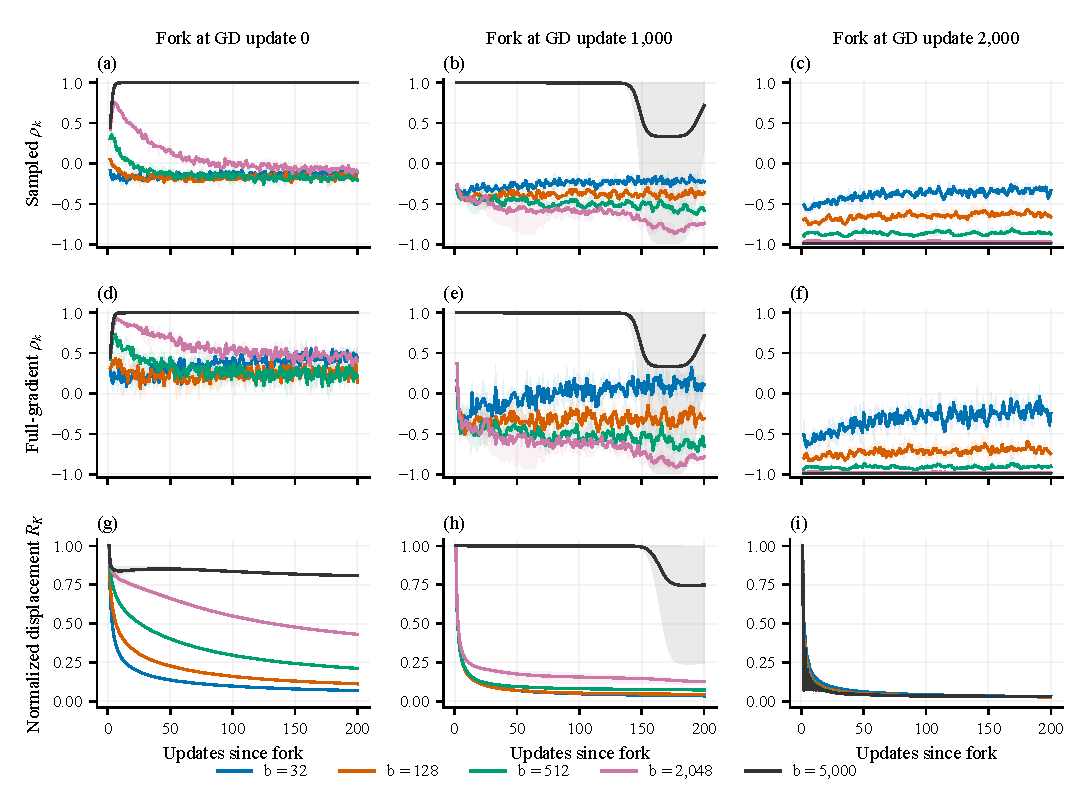
\includegraphics[width=\textwidth]{figures/analysis027/sgd_geometry_raw.pdf}
  \caption{Unsmoothed counterpart of Fig.~\ref{fig:sgd-moving-geometry}.
  Cosines retain every defined adjacent pair. Curves and shading use the
  same repetition means and descriptive range across three initializations;
  no temporal averaging is applied.}
  \label{fig:sgd-raw-geometry}
\end{figure*}

\begin{figure*}[!t]
  \centering
  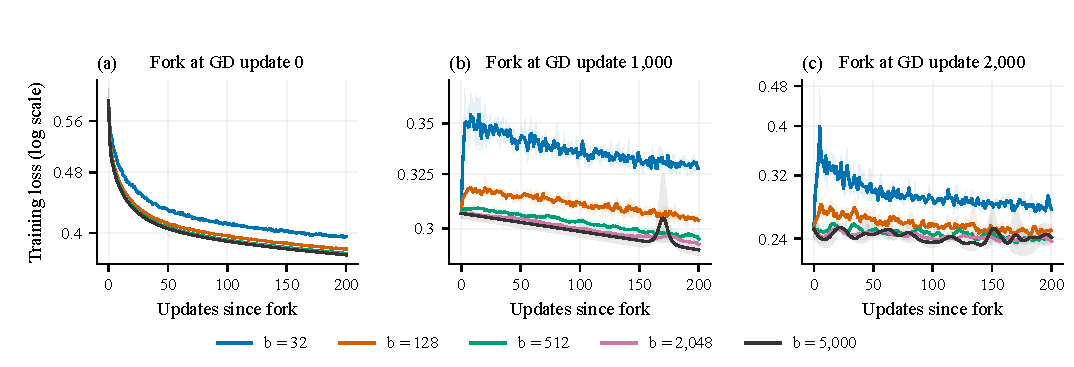
\includegraphics[width=\textwidth]{figures/analysis027/sgd_full_loss.pdf}
  \caption{Complete-objective training loss along the same continuations,
  with logarithmic vertical axes and no temporal smoothing. Columns denote
  the shared fork checkpoint. Curves first average the sampling repetitions
  within each initialization; lines and shading then show the mean and
  range of the three initialization means. Every value covers all 5,000
  training images, including the final update.}
  \label{fig:sgd-full-loss}
\end{figure*}

\subsection{Noise Correction and Directional Curvature}

Write $\mu_k=\nabla\mathcal L(\theta_{k-1})$ and
$q_k=\eta\widehat\kappa_k$ within each continuation. With the measured
$\xi_k=g_k-\mu_k$, the following finite-step identity holds:
\begin{equation}
  q_k+\varepsilon_k
  =\frac{g_{k-1}^{\top}(\mu_{k-1}-\mu_k)}{\|g_{k-1}\|^2}.
  \label{eq:sgd-corrected-projection}
\end{equation}
Agreement with this identity checks accounting, not the curvature
approximation. We separately evaluate complete-objective Hessian--vector
products at the states preceding gradients 1, 51, 101 and 151, using the
sampled gradient as direction. These yield $\eta\kappa_k$ for the
following pairs, at indices 2, 52, 102 and 152. All 5,000 training examples
contribute; no spectral subset or maximum-eigenvalue estimate is used.

Table~\ref{tab:sgd-hvp-errors} compares the raw proxy and noise-corrected
projection with these 1,188 state-matched directional-HVP values.
Residuals are calculated from unsmoothed paired observations. Correcting
the explicit noise-difference term leaves the sampled direction, visited
state and finite-step Taylor remainder intact.
This correction is an offline reference requiring complete gradients;
it is not available from two sampled gradients alone.

\begin{table}[!t]
  \centering
  \caption{Absolute error against the state-matched directional value
  $\eta\kappa_k$. Raw uses $q_k$; corrected uses $q_k+\varepsilon_k$.
  Medians and 90th percentiles pool the four probe pairs per continuation
  across all three initializations and checkpoints. These are descriptive
  errors in the measured directions, not independent-pair confidence intervals.}
  \label{tab:sgd-hvp-errors}
  \small
  \begin{tabular}{rrrrr}
\hline
$b$ & Pairs & Raw med. & Corr. med. & Corr. 90th \\
\hline
32 & 288 & 0.7467 & 0.0030 & 0.0143 \\
128 & 288 & 0.5648 & 0.0033 & 0.0163 \\
512 & 288 & 0.3914 & 0.0034 & 0.0205 \\
2,048 & 288 & 0.1759 & 0.0025 & 0.0224 \\
5,000 & 36 & $<0.0001$ & $<0.0001$ & 0.0218 \\
\hline
\end{tabular}

\end{table}

\begin{figure*}[!t]
  \centering
  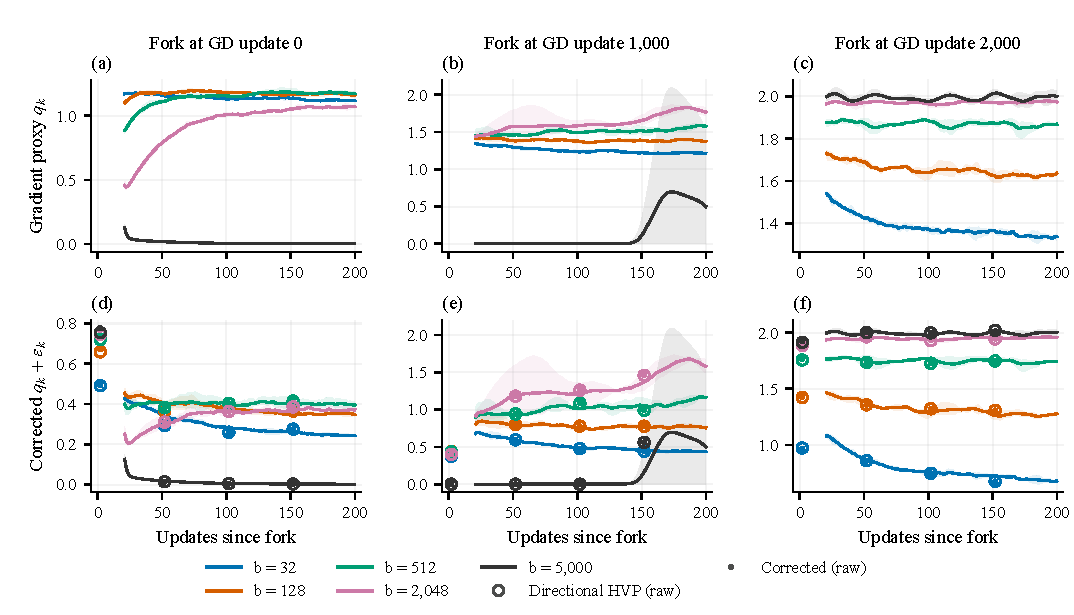
\includegraphics[width=\textwidth]{figures/analysis027/sgd_proxy_validation.pdf}
  \caption{Observed gradient-change proxy (top) and noise-corrected
  projection (bottom) on the moving trajectories. Curves use complete
  20-pair trailing means, followed by the same repetition/initialization
  reduction as Fig.~\ref{fig:sgd-moving-geometry}. At the four probe pairs,
  filled dots show raw corrected projections and open circles show their
  state-matched directional-HVP values, averaged across repetitions and
  initializations. Markers retain the raw pair; curves provide smoothed
  temporal context. Quantitative errors use the individual raw paired values in
  Table~\ref{tab:sgd-hvp-errors}.}
  \label{fig:sgd-proxy-validation}
\end{figure*}
